\section{Resultados}

\subsection{Acto 1: las fusiones empatan en validación}

La Tabla~\ref{tab:acto1} repite la tabla de la entrega parcial. Frente a A, la diferencia pareada de \dmas{} es $-0{,}009$ para B (IC95 $-0{,}055$ a $+0{,}024$; $p=0{,}52$), $-0{,}009$ para C ($-0{,}061$ a $+0{,}030$; $p=0{,}87$) y $+0{,}018$ para E ($-0{,}020$ a $+0{,}062$; $p=0{,}93$). Los tres intervalos cruzan el cero. Todas las redes, en cambio, dejan 57 veces menos falso positivo que el umbral clásico, con un \dmas{} tres veces y media mayor. Por diagnóstico, el patrón se repite en todos los brazos: pulmón cerca de 0,74, linfoma 0,70 y melanoma 0,40.

\begin{table}[h]
\centering\small
\caption{Acto 1, validación (26 estudios, 20 positivos evaluables). Media $\pm$ desviación entre tres semillas. \texttt{mejor.pt} es el checkpoint del protocolo; \texttt{ultimo.pt}, la iteración 25\,000.}
\label{tab:acto1}
\begin{tabular}{lcccccc}
\toprule
 & \multicolumn{3}{c}{\texttt{mejor.pt}} & \multicolumn{3}{c}{\texttt{ultimo.pt}} \\
\cmidrule(lr){2-4}\cmidrule(lr){5-7}
Brazo & \dmas & FPV (mL) & FNV (mL) & \dmas & FPV (mL) & FNV (mL) \\
\midrule
A & 0,621 $\pm$ 0,016 & 20,9 $\pm$ 2,5 & 6,0 & 0,615 $\pm$ 0,020 & 21,7 $\pm$ 0,5 & 5,9 \\
B & 0,612 $\pm$ 0,014 & 22,8 $\pm$ 3,1 & 5,4 & 0,607 $\pm$ 0,002 & 22,1 $\pm$ 2,8 & 4,4 \\
C & 0,612 $\pm$ 0,008 & 23,2 $\pm$ 6,7 & 5,9 & 0,610 $\pm$ 0,007 & 21,5 $\pm$ 1,8 & 4,5 \\
E & 0,640 $\pm$ 0,022 & 22,0 $\pm$ 9,8 & 7,3 & 0,638 $\pm$ 0,006 & 23,6 $\pm$ 2,8 & 5,7 \\
Clásica & 0,180 & 1\,191,9 & 5,6 & & & \\
\bottomrule
\end{tabular}
\end{table}

\textbf{La atención de C quedó inerte.} Al forzar $\gamma=0$ en el modelo entrenado, la predicción no cambió en un solo vóxel: diferencia de Dice 0,000 en los 26 estudios y en las tres semillas. Medí por qué. Los pesos de atención resultaron casi uniformes sobre las 216 posiciones, de modo que cada posición del PET recibía casi el mismo vector, un promedio de todo el CT. La salida de la atención era en un 99\,\% constante en el espacio. La convolución que sigue tiene normalización de instancia, que resta a cada canal su media espacial, y una señal igual en todas las posiciones desaparece.

\textbf{El canal de E está vivo, pero no paga.} Al reemplazar la referencia hepática del paciente por una constante poblacional (2,165, la mediana de los 176 de entrenamiento), cambian 23 de 26 predicciones, pero el efecto neto sobre el FPV es de 1,4 mL, menor que la variación entre semillas. Su ventaja aparente venía del checkpoint: el protocolo había elegido la iteración 9\,000.

\textbf{El checkpoint pesa más que la semilla.} \texttt{mejor.pt} se elige con el máximo Dice de una validación rápida de 12 estudios, una curva muy ruidosa (Figura~\ref{fig:curvas}). Al usar el checkpoint final, la desviación del FPV entre semillas baja 5,1 veces en A, 3,8 en C y 3,4 en E, mientras el Dice medio cambia 0,005 y el orden entre modelos se mantiene. Elegir el máximo de una curva ruidosa optimiza una métrica y deja las otras al azar.

\begin{figure}[h]
\centering
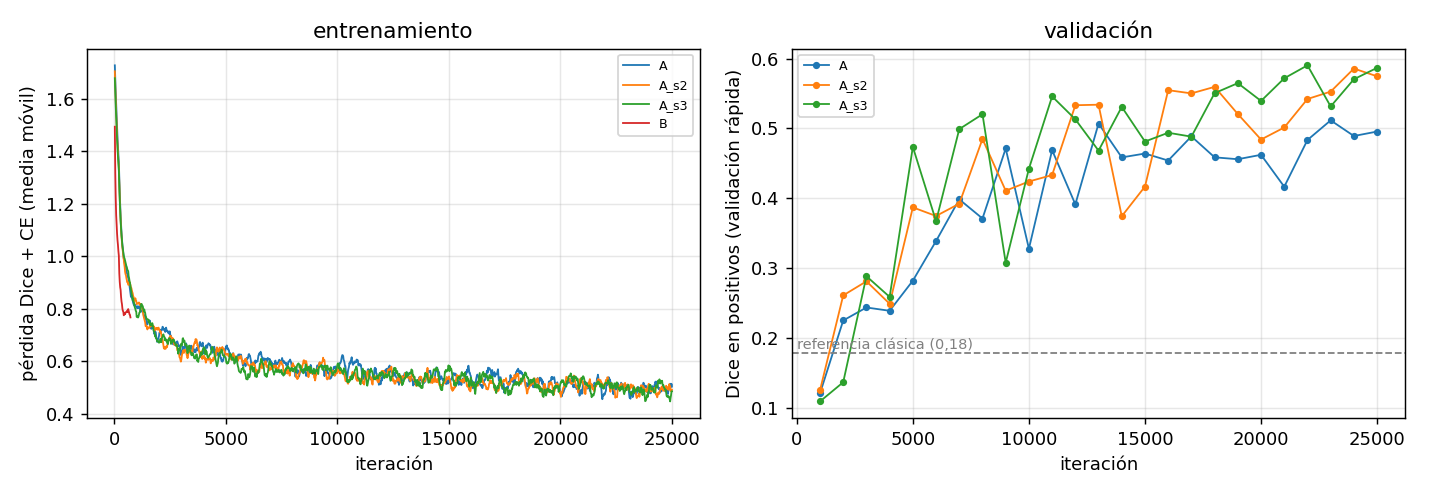
\includegraphics[width=\linewidth]{curvas_entrenamiento.png}
\caption{Acto 1: pérdida de entrenamiento (izquierda) y Dice de la validación rápida de 12 estudios (derecha) en las doce corridas. La pérdida baja igual en todos los brazos. La curva de validación salta de un punto a otro, y elegir su máximo como checkpoint introduce ruido en el falso positivo.}
\label{fig:curvas}
\end{figure}

\subsection{Etapa extendida: el empate era falta de entrenamiento}

\textbf{Paso 1, datos o tiempo.} Cuadruplicar las iteraciones mejoró el \dmas{} de A en +0,041 y +0,045, ganando en 17 de 20 estudios las dos veces (Tabla~\ref{tab:2x2}). Quintuplicar los estudios con las iteraciones fijas no movió nada claro: con 25\,000 iteraciones y 825 estudios, cada estudio se veía en promedio 61 veces en vez de 284. El cuello de botella del acto 1 era cuánto entrenaba la red.

\begin{table}[h]
\centering\small
\caption{Paso 1, diseño 2\,×\,2 con el brazo A (validación, una semilla).}
\label{tab:2x2}
\begin{tabular}{lccc}
\toprule
 & \dmas & FPV (mL) & FNV (mL) \\
\midrule
176 estudios, 25\,000 iteraciones & 0,615 & 21,7 & 5,9 \\
176 estudios, 100\,000 iteraciones & 0,655 & 15,5 & 5,2 \\
825 estudios, 25\,000 iteraciones & 0,636 & 24,7 & 5,1 \\
825 estudios, 100\,000 iteraciones & 0,681 & 15,8 & 3,9 \\
\bottomrule
\end{tabular}
\end{table}

\textbf{Paso 2, las arquitecturas con entrenamiento suficiente.} Con 825 estudios y 100\,000 iteraciones, los brazos de doble codificador quedaron arriba (Tabla~\ref{tab:paso2}): el orden del acto 1 se invirtió. A+, con los mismos parámetros que B, empató con A. En validación, con 20 positivos, la ventaja de B sobre A con tres semillas fue de +0,012, con un intervalo que cruzaba el cero. La atención de C siguió inerte: $\gamma$ terminó en 0,992 y la ablación volvió a dar cero en las tres semillas.

\begin{table}[h]
\centering\small
\caption{Paso 2, validación, 825 estudios y 100\,000 iteraciones, media de tres semillas.}
\label{tab:paso2}
\begin{tabular}{lccc}
\toprule
Brazo & Parámetros & \dmas & FPV (mL) \\
\midrule
A & 12,9 M & 0,694 & 15,1 \\
A+ & 24,3 M & 0,694 & 15,8 \\
B & 24,0 M & 0,705 & 13,3 \\
C & 24,4 M & 0,713 & 13,2 \\
\bottomrule
\end{tabular}
\end{table}

\textbf{Paso 3, enseñar anatomía no cumplió sus criterios.} Con B, el falso positivo en órganos fisiológicos ya era solo el 18\,\% del total; el resto estaba en tejido sin etiqueta, pulmón y bordes. El codificador del CT preentrenado aprendió los 17 grupos de órganos con un Dice anatómico de 0,861, y B partiendo de él dio con una semilla el mejor Dice de todas las corridas largas, 0,724. Antes de correr más declaré una hipótesis nueva: aceptarlo solo si las semillas 2 y 3 daban ambas 0,716 o más. Dieron 0,700 y 0,698. Con tres semillas, B preentrenada quedó en 0,707 frente a 0,705 de B ($p=0{,}78$). La pérdida pesada por órgano tampoco cumplió su criterio.

\textbf{Paso 4, el ensamble.} En validación, B solo dio \dmas{} 0,706 y 13,3 mL de FPV; el ensamble, 0,744 y 10,0 mL; el ensamble con TTA, 0,754 y 9,2 mL. El criterio fijado antes era FPV menor que 9 mL y no se cumplió, pero contra B la mejora fue significativa en Dice (+0,048, IC95 +0,024 a +0,079) y en FPV ($-4{,}0$ mL, IC95 $-6{,}6$ a $-2{,}2$). Detectó las mismas lesiones que B (160 de 256) con la mitad de marcas falsas por estudio (2,8 contra 4,8 a 5,8). La predicción fuera de pliegue de los 825 estudios dio \dmas{} 0,689, la primera medición del proyecto sobre más de 26 estudios.

\textbf{El umbral y la regla del hígado.} En los 825 estudios fuera de pliegue el \dmas{} era casi plano entre umbrales (0,698 a 0,699), mientras en los 26 de validación subía de 0,754 a 0,784 entre 0,5 y 0,7: esa subida era ruido de 26 estudios. La regla eligió 0,6. La regla del hígado bajó las marcas falsas un 22\,\% y perdió el 6,4\,\% de las lesiones, así que no se adoptó.

\subsection{La prueba}

\textbf{Las dos hipótesis se confirman} (Tabla~\ref{tab:h}). El falso positivo baja en los 49 estudios, sin excepción. El sistema final queda en \dmas{} 0,727 (mediana 0,806), FPV 9,5 mL y FNV 3,95 mL; con la métrica cruda del reto, en \dmas{} 0,705 y FPV 9,5 mL. Por diagnóstico, su \dmas{} medio es 0,721 en pulmón, 0,749 en linfoma y 0,709 en melanoma.

\begin{table}[h]
\centering\small
\caption{Hipótesis preregistradas, prueba (49 estudios, 38 positivos). Diferencias pareadas contra B extendido (media de tres semillas).}
\label{tab:h}
\begin{tabular}{lcccc}
\toprule
 & $\Delta$\dmas & IC95 & $\Delta$FPV (mL) & IC95 \\
\midrule
H1, ensamble + TTA, umbral 0,5 & +0,028 & +0,011 a +0,048 & $-7{,}0$ & $-12{,}4$ a $-3{,}4$ \\
H2, sistema final, umbral 0,6 & +0,029 & +0,006 a +0,054 & $-9{,}4$ & $-16{,}4$ a $-4{,}5$ \\
\bottomrule
\end{tabular}
\end{table}

La Tabla~\ref{tab:prueba} muestra todos los brazos. Tres lecturas:
\begin{itemize}
\item \textbf{El acto 1 se sostiene en Dice.} B, C y E contra A tienen intervalos que cruzan el cero. En FPV, B y C bajan la media de A unos 14 mL con intervalos que no cruzan el cero, pero Wilcoxon no sale significativo y el FPV baja en menos de la mitad de los estudios. La media de A (38,4 mL, mediana 13,2) la arrastran cuatro estudios donde marcó más de 200 mL. Los dos codificadores evitan algunos fallos grandes de la fusión temprana, pero no mejoran el estudio típico, y como B lo hace igual que C, nada de esto se puede atribuir a la atención.
\item \textbf{Con entrenamiento suficiente, la fusión intermedia gana.} En el extendido, B supera a A en \dmas{} (+0,038, IC95 +0,006 a +0,076) y en FPV ($-7{,}7$ mL, IC95 $-16{,}9$ a $-1{,}6$), y C hace lo mismo (+0,034 y $-7{,}6$ mL). A+ no se distingue de A (+0,001, IC95 $-0{,}007$ a $+0{,}009$). La ventaja no es por tamaño. Lo que en validación no alcanzaba a verse con 20 positivos se ve con 38.
\item \textbf{El ensamble es la mejora más grande y más sólida.} Contra sus propios cinco miembros, el ensamble con TTA gana +0,029 (IC95 +0,019 a +0,041) en 34 de 38 positivos.
\end{itemize}

\begin{table}[h]
\centering\small
\caption{Todos los brazos en la prueba, métrica corregida. Media de tres semillas salvo donde se indica.}
\label{tab:prueba}
\begin{tabular}{lccccc}
\toprule
Brazo & \dmas & mediana & FPV (mL) & FNV (mL) & FPV en controles \\
\midrule
Clásica (SUV $\geq 2{,}5$) & 0,182 & 0,128 & 832,5 & 2,1 & 987,1 \\
\addlinespace
Acto 1 · A & 0,616 & 0,664 & 38,4 & 5,8 & 85,7 \\
Acto 1 · B & 0,630 & 0,676 & 23,6 & 5,5 & 45,0 \\
Acto 1 · C & 0,607 & 0,633 & 24,8 & 6,9 & 48,5 \\
Acto 1 · E & 0,596 & 0,644 & 28,6 & 8,8 & 58,4 \\
\addlinespace
Extendido · A & 0,660 & 0,717 & 26,6 & 3,6 & 39,6 \\
Extendido · A+ & 0,662 & 0,714 & 23,5 & 4,6 & 39,4 \\
Extendido · B & 0,698 & 0,742 & 18,9 & 2,7 & 29,1 \\
Extendido · C & 0,695 & 0,734 & 18,9 & 2,6 & 29,3 \\
Extendido · B preentrenada & 0,709 & 0,758 & 16,3 & 3,1 & 25,7 \\
\addlinespace
Ensamble + TTA, umbral 0,5 (H1) & 0,726 & 0,798 & 11,9 & 3,5 & 13,8 \\
\textbf{Sistema final, umbral 0,6 (H2)} & \textbf{0,727} & \textbf{0,806} & \textbf{9,5} & \textbf{3,95} & \textbf{9,6} \\
\bottomrule
\end{tabular}
\end{table}

\textbf{Dónde queda el error.} La Figura~\ref{fig:fporg} reparte el falso positivo por órgano. El umbral clásico pone su error en órganos de captación fisiológica: hígado 167, riñones 111, vejiga 110, corazón 107 e intestino 90 mL por estudio. Las redes dejan menos de 1 mL en hígado, riñones, vejiga y corazón. Lo que les queda está en tejido sin órgano asignado, hueso, bazo y el borde del cuerpo, y el sistema final baja cada uno de esos grupos a menos de 3 mL.

\begin{figure}[h]
\centering
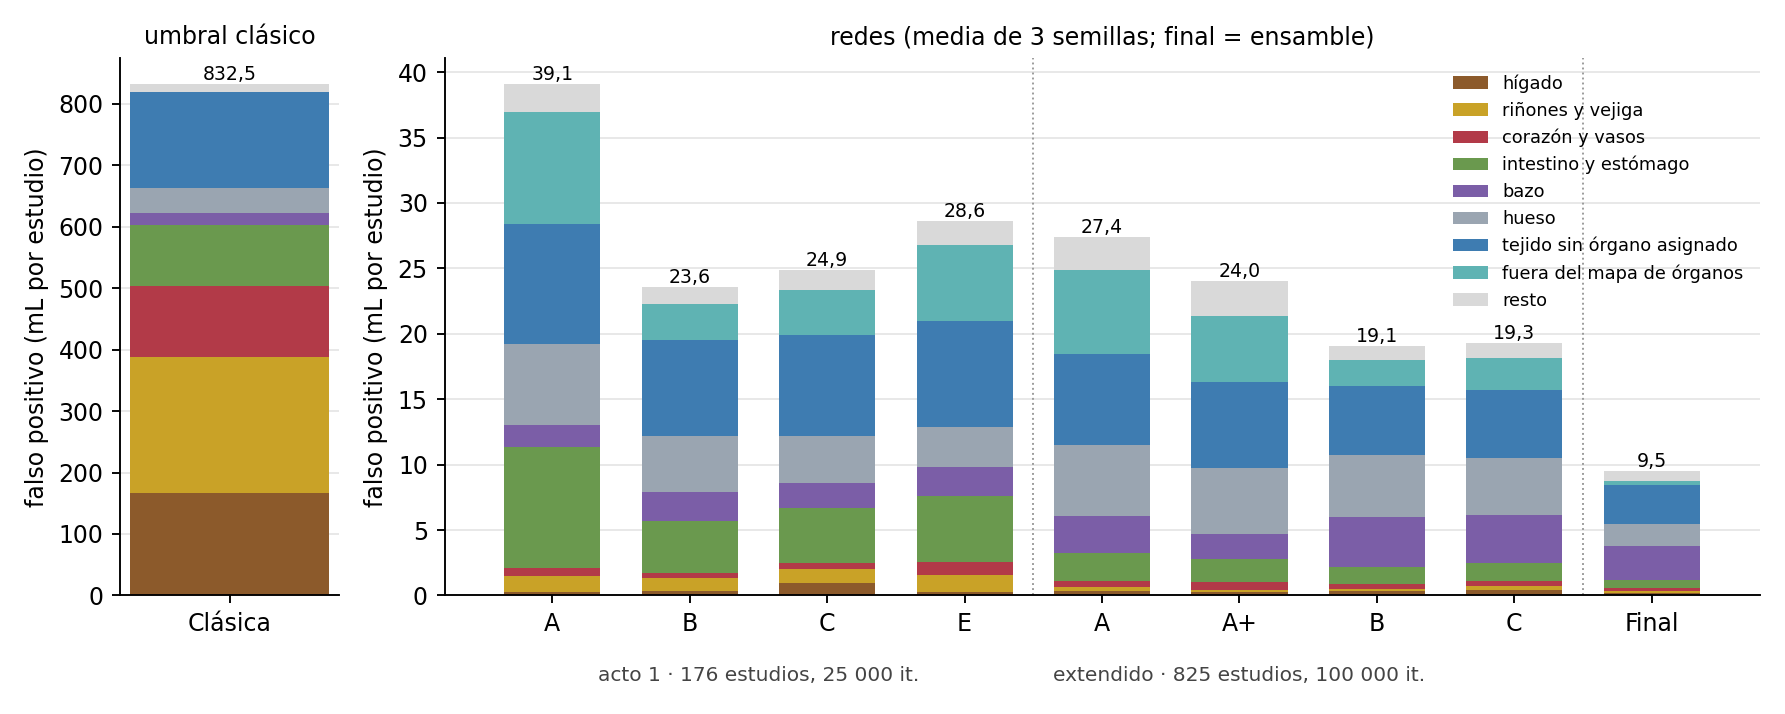
\includegraphics[width=\linewidth]{fp_por_organo_test.png}
\caption{Falso positivo por órgano en la prueba (mL por estudio, incluida la zona anonimizada, por eso A del acto 1 suma 39,1 y no 38,4). Izquierda, el umbral clásico en su propia escala; derecha, las redes. Los grupos vienen del mapa de órganos de TotalSegmentator sobre el CT.}
\label{fig:fporg}
\end{figure}

\textbf{Por lesión.} De las 435 lesiones de la prueba, el ensamble detecta 330, lo mismo que un B solo (327 a 337), con 7,8 marcas falsas por estudio en vez de 12,8 a 13,6. El sistema final baja a 6,3 marcas a cambio de 8 lesiones menos (322). Se detectan casi todas las lesiones de más de 10 mL y la mitad de las de menos de 1 mL.

\textbf{Casos.} La Figura~\ref{fig:casos} muestra cuatro estudios de la prueba elegidos con una regla fija, escrita antes de mirar las imágenes, sobre las métricas del sistema final: el caso típico (Dice más cercano a la mediana), el de mayor FPV, el de mayor FNV y el de mayor corrección del ensamble frente a B. En el caso típico (A), el umbral clásico pinta la columna, la médula y la vejiga, y las redes no. En el de mayor FPV (B), un linfoma, el error de las redes cae sobre todo en el bazo, donde la captación puede ser enfermedad no anotada. En el de mayor FNV (C), el sistema final pierde varias lesiones pequeñas que B sí tocaba: 26,0 contra 8,8 mL, el costo del umbral 0,6 visto en un paciente. En el control (D), el ensamble baja el FPV de B de 171 a 66 mL, y lo que queda está en la pelvis.

\begin{figure}[p]
\centering
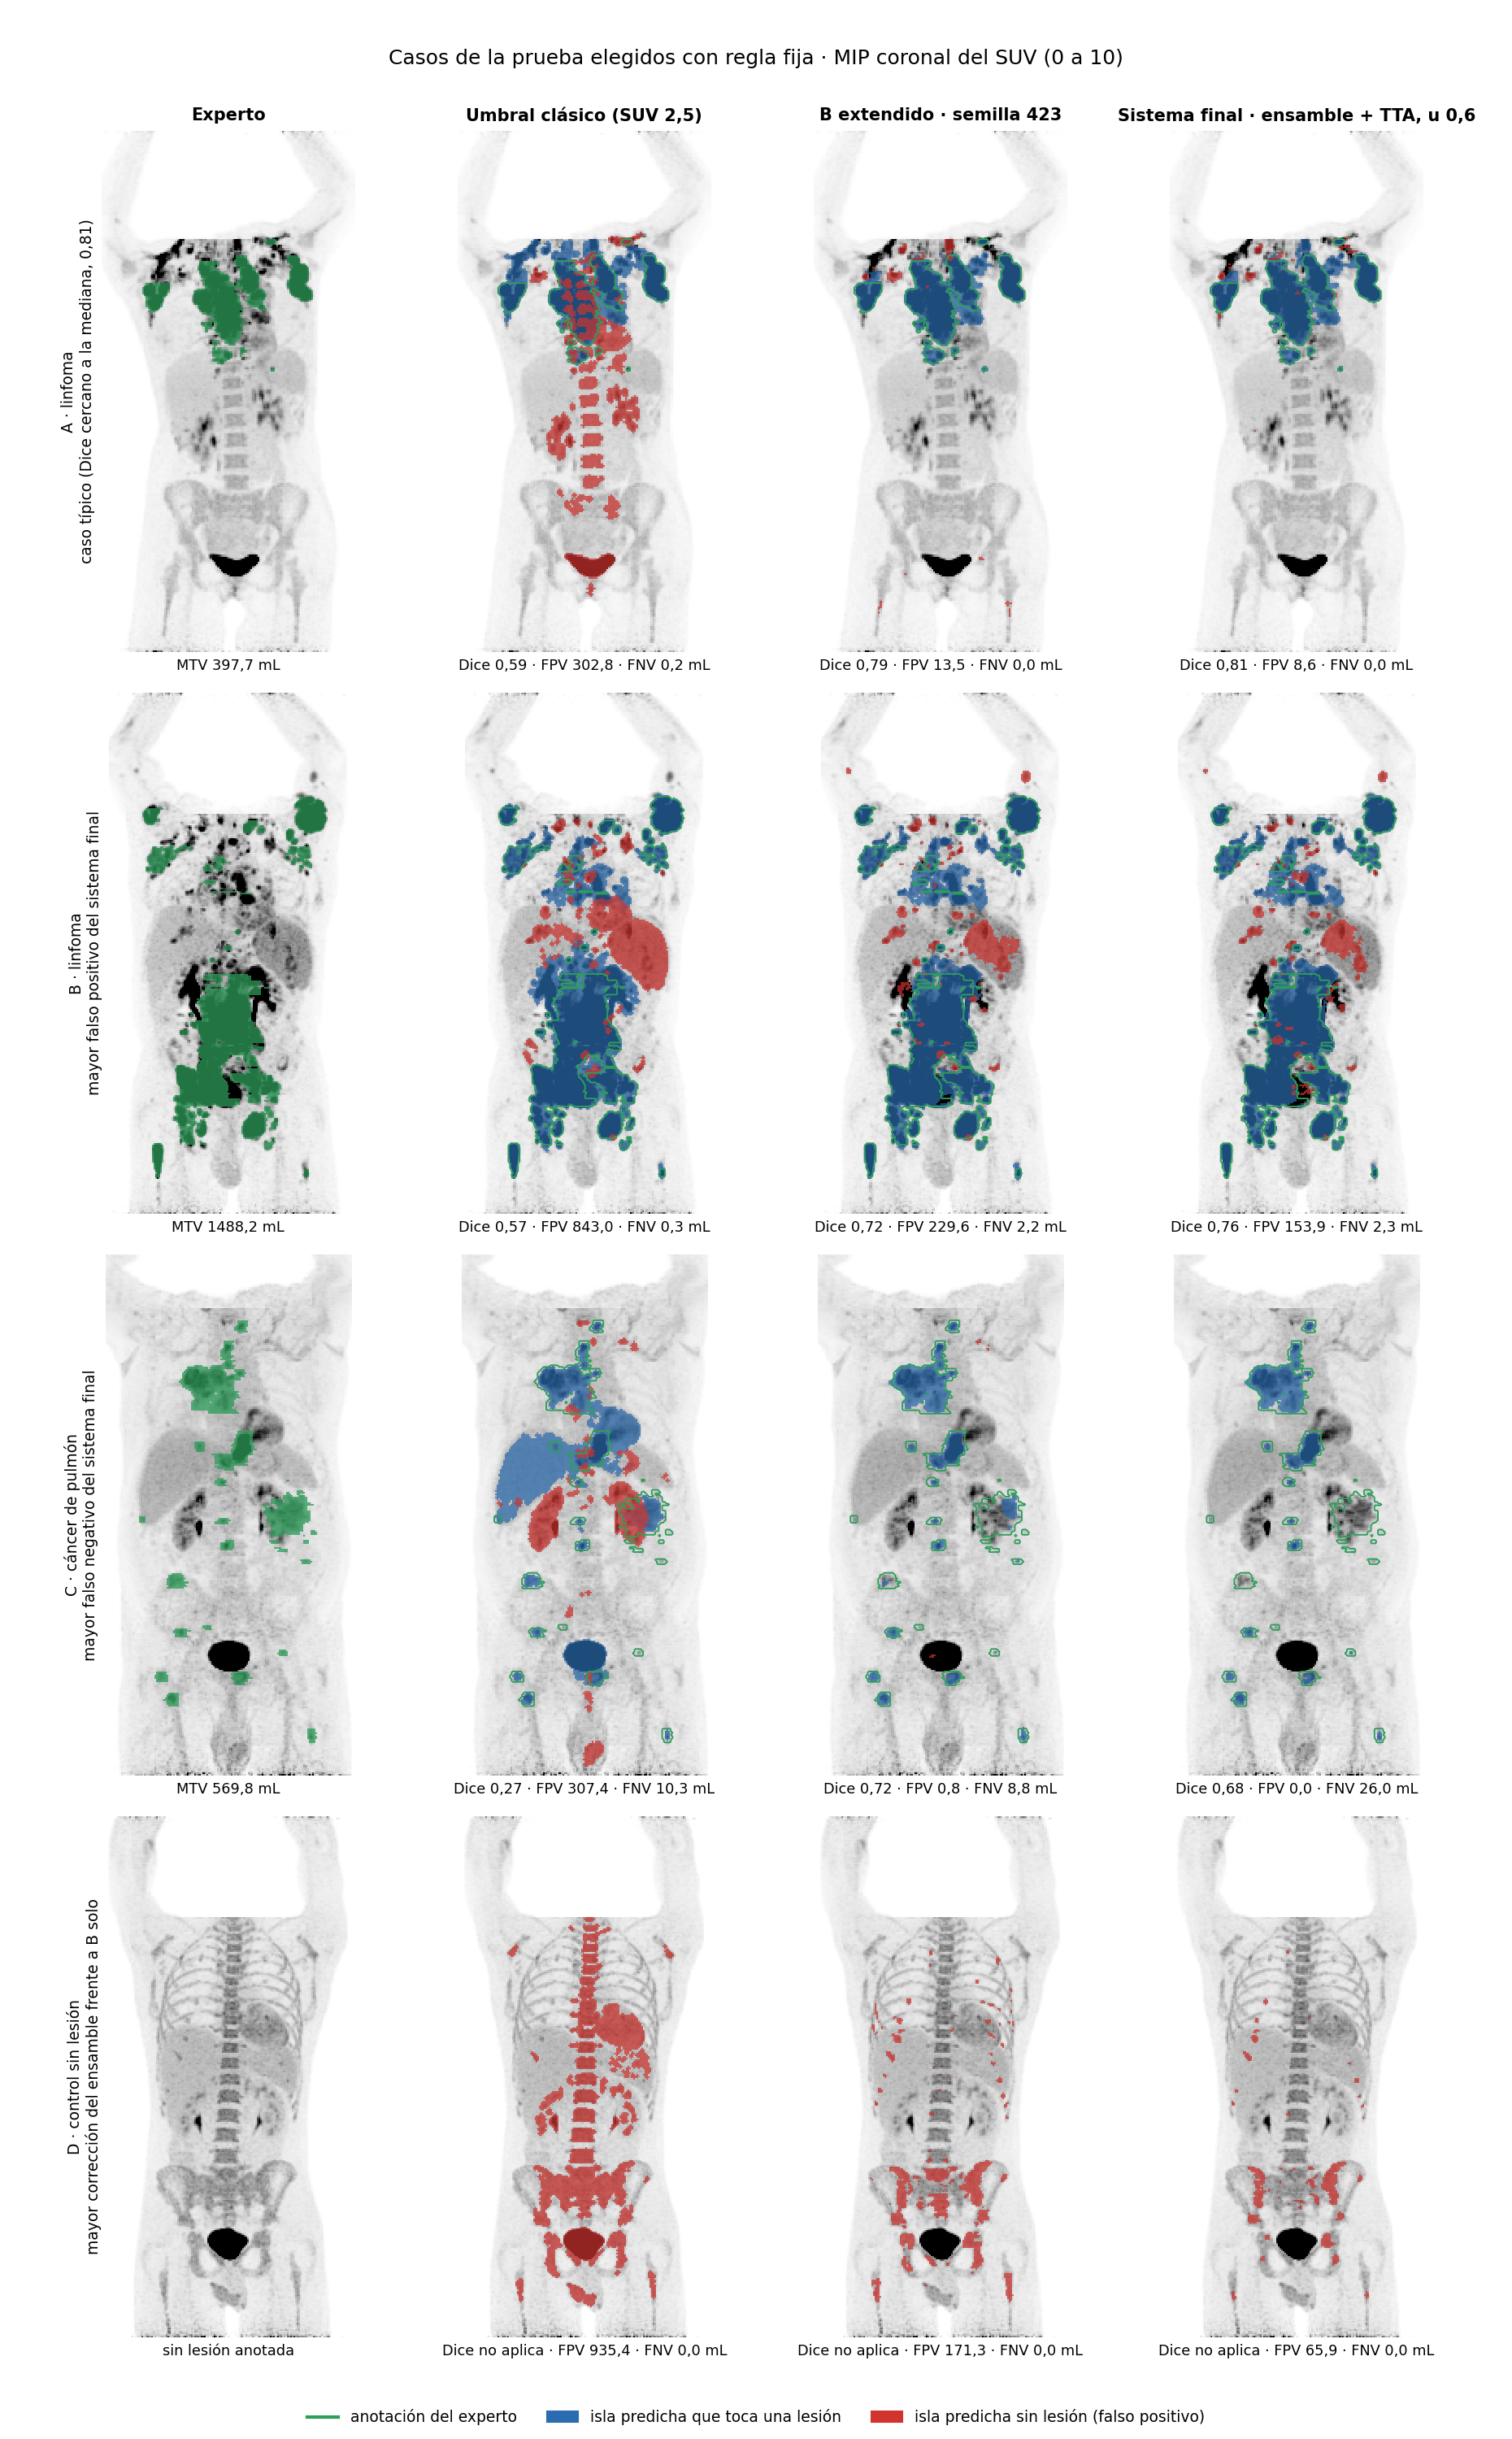
\includegraphics[height=0.86\textheight,keepaspectratio]{casos_test.png}
\caption{Casos de la prueba elegidos con regla fija (\texttt{scripts/42}). MIP coronal del SUV (0 a 10). Verde, anotación del experto; azul, islas predichas que tocan una lesión; rojo, islas predichas sin lesión. Bajo cada panel, las métricas de ese estudio.}
\label{fig:casos}
\end{figure}

\subsection{Análisis secundarios}
\label{sec:secundarios}

Estos análisis estaban comprometidos en la definición de tema pero no en el preregistro de la prueba. Los calculé después de abrirla, sobre las máscaras ya guardadas y sin parámetros ajustables, y no cambian los veredictos de H1 y H2.

\textbf{Hausdorff 95.} En los 38 positivos, la mediana del HD95 es 252,9 mm para la clásica, 93,3 para A del acto 1, 64,1 para B extendido, 31,0 para el ensamble con TTA y 23,5 para el sistema final. Contra B, el sistema final lo baja 16,5 mm (IC95 $-26{,}2$ a $-0{,}7$; mejora en 27 de 38; $p<0{,}001$). Entre arquitecturas no hay diferencia. El HD95 castiga mucho las islas falsas lejanas, y por eso el ensamble, que deja menos marcas falsas, es lo que más lo baja.

\textbf{SUVmax.} En el sistema final el error mediano del SUVmax por paciente es cero y el 87\,\% de los pacientes queda dentro de un 10\,\%, contra 79\,\% de B y 32\,\% de la clásica. De los cinco que quedan fuera, en cuatro la predicción da un SUVmax mayor: marcó algo más caliente que la lesión. Hay dos límites: el preprocesamiento pone tope al SUV en 30, y 4 de los 38 estudios tienen el SUVmax anotado en ese tope; y el SUVmax se mide en la grilla de 3 mm.

\textbf{Script oficial de autoPET.} Sobre las mismas máscaras, en la métrica cruda, el Dice sale idéntico. El oficial cuenta componentes con conectividad 18 y el mío con 26; en las redes, el FPV y el FNV difieren en 3 a 7 de 49 estudios y nunca en más de 0,62 mL. Solo en el umbral clásico, que deja cientos de islas, la diferencia llega a 36 mL en un estudio. Ninguna conclusión cambia.

\textbf{Clásica con exclusión de órganos.} Apagando las islas que caen en más de la mitad dentro de 12 grupos de órganos de captación fisiológica (lista fijada el 24 de septiembre, antes de abrir la prueba), la clásica sube de \dmas{} 0,182 a 0,379 y baja el FPV de 832,5 a 94,8 mL, pero el FNV sube de 2,1 a 28,6 mL porque también apaga metástasis hepáticas y ganglios que el mapa asigna a vasos o corazón. Aun así deja diez veces el FPV del sistema final.
